\section{Дослідження алгоритму оптимальної фільтрації за допомогою розробленого програмного забезпечення}
В роботі проведено дослідження розроблених алгоритмів оптимальної калманівської фільтрації, в результаті розроблено програмне забезпечення. Дослідження проведені шляхом моделювання еволюцій похибок БІНС та СНС, та їх оцінки за допомогою оптимального рекурентного фільтра Калмана. Програмне розроблене на об'єктно-орієнтовній мові програмування Java, основною перевагою якої є незалежність від архітектури.

Розробка проведена в середовищі Java SE 6 (1.6.0). У офіційній реалізації, Java програми компілюються у байткод, який при виконанні інтерпретується віртуальною машиною для конкретної платформи. Sun Microsystems надає компілятор Java та віртуальну машину Java, які задовольняють специфікації Java Community Process, під ліцезією GNU General Public License. 

Під «незалежністю від архітектури» мається на увазі те, що програма, написана на мові Java, працюватиме на будь-якій підтримуваній апаратній чи системній платформі без змін у початковому коді та перекомпіляції.

Цього можна досягти, компілюючи початковий Java код у байт-код, який являє собою спрощені машинні команди. Потім програму можна виконати на будь-якій платформі, що має встановлену віртуальну машину Java, яка інтерпретує байткод у код, пристосований до специфіки конкретної операційної системи і процесора. Зараз віртуальні машини Java існують для більшості процесорів і операційних систем, в тому числі різноманітних версій GNU/Linux, Microsoft Windows, Apple Mac OS, мобільних платформ, наприклад Google Android та багато інших.

В програмі використані наступні бібліотеки:
\begin{itemize}
  \item JMathPlot - побудова графіків;
  \item JMathArray(JAMA) - математичні розрахунки;
  \item JMathIO - зберігання/читання даних в ASCII форматі;
  \item Swing - розробка графічного інтерфейсу.
\end{itemize}

Математичні обчислення проводяться за допомогою спеціалізованої бібліотеки JAMA. Це програмна бібліотека для розв'язання задач лінійної алгебри. Ця бібліотека створена Національним інститутом стандартів і технологій США і схожа по функціональності з LAPACK. Існують версії JAMA для мов програмування C++ та Java.Іншою перевагою є те, що ця бібліотека розповсюджується вільно, з багатою документацією та джерельними кодами.

Swing -- інструментарій для створення графічного інтерфейсу користувача (GUI) мовою програмування Java. Це частина бібліотеки базових класів Java (JFC, Java Foundation Classes). Дозволяє зручна та швидко створити інтерфейс користувача будь якої складності.

JMathPlot, JMathIO -- зручні бібліотеки, що розповсюджуються під ліцензією BSD, для виводу графічної інформації: гістограм, 2D та 3D графіків.

\subsection{Опис вхідних та вихідних даних}
Вхідними даними для програми є параметри інтегрування, параметри руху ЛА, параметри БІНС: початкові похибки гіроскопів, акселерометрів, барометричного висотоміра та параметри СНС: випадкові та корельовані складові похибок по кожному каналу. 

Через дружній графічний інтерфейс, користувач має можливість ввести або змінити наступні данні:
\begin{itemize}
  \item час моделювання;
  \item крок розрахунку;
  \item параметри траєкторії руху ЛА:
  \item початкові координати;
  \item лінійні і гармонічні складові траєкторії по кожному каналу;
  \item дрейф та випадкове блукання гіроскопа;
  \item похибка барометричного висотоміра;
  \item кореляційна матриця системи
  \item кореляційні похибки СНС;
  \item випадкові похибки СНС;
\end{itemize}
Вихідні данні представлені у вигляді графіків, або існує можливість зберегти їх в текстовому файлі, яким можна потім наприклад завантажити в середовище Octave чи Matlab. Отже на виході отримується наступна інформація: 
\begin{itemize}
  \item оцінки координат;
  \item оцінки швидкостей;
  \item оцінки зміщення навігаційного тригранника;
  \item оцінки дрейфів гіроскопів;
  \item оцінка зміщення акселерометрів.
\end{itemize}
За допомогою графічного інтерфейсу, користувач має можливість наочно отримати результати розрахунків, або імпортувати в іншу підпрограму чи середовище розробки.

\subsection{Опис графічного інтерфейсу користувача}

Інтерфейс програми складається з вікна програми, яке включає поля для введення параметрів траєкторії руху ЛА, меню та закладки з графічною інформацією. На Рис.\ref{fig:3d_soft} зображено головне вікно, з графіком траєкторії руху ЛА.

\begin{figure}[t]
\centering
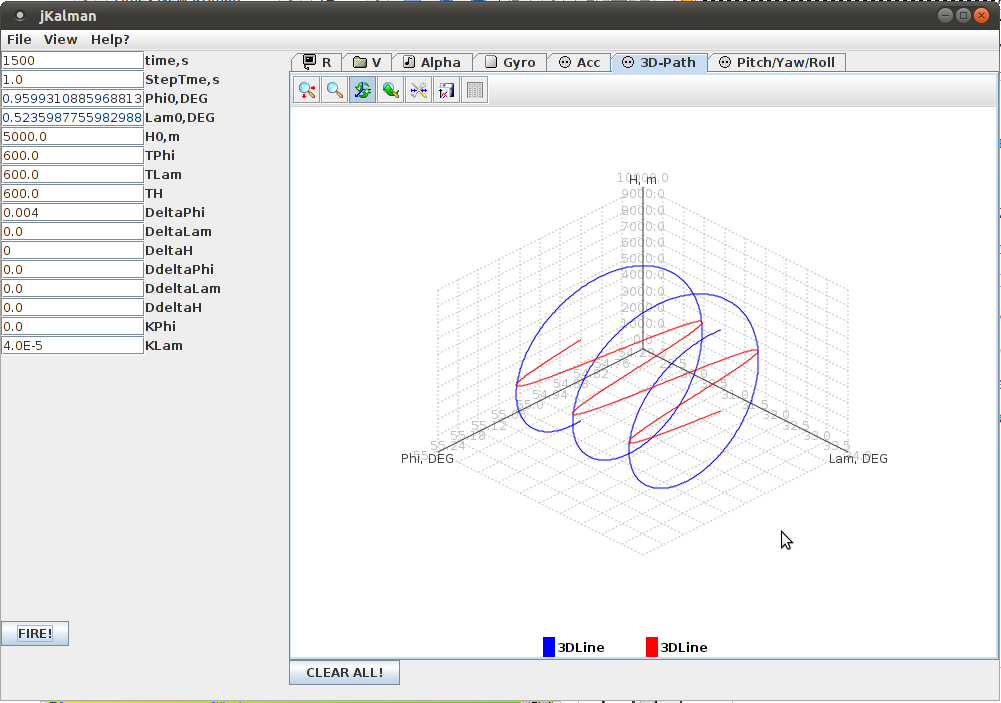
\includegraphics[scale=0.4]{3d_soft}
\caption{Головне вікно програми}\label{fig:3d_soft}
\end{figure}

\begin{figure}[t]
\centering
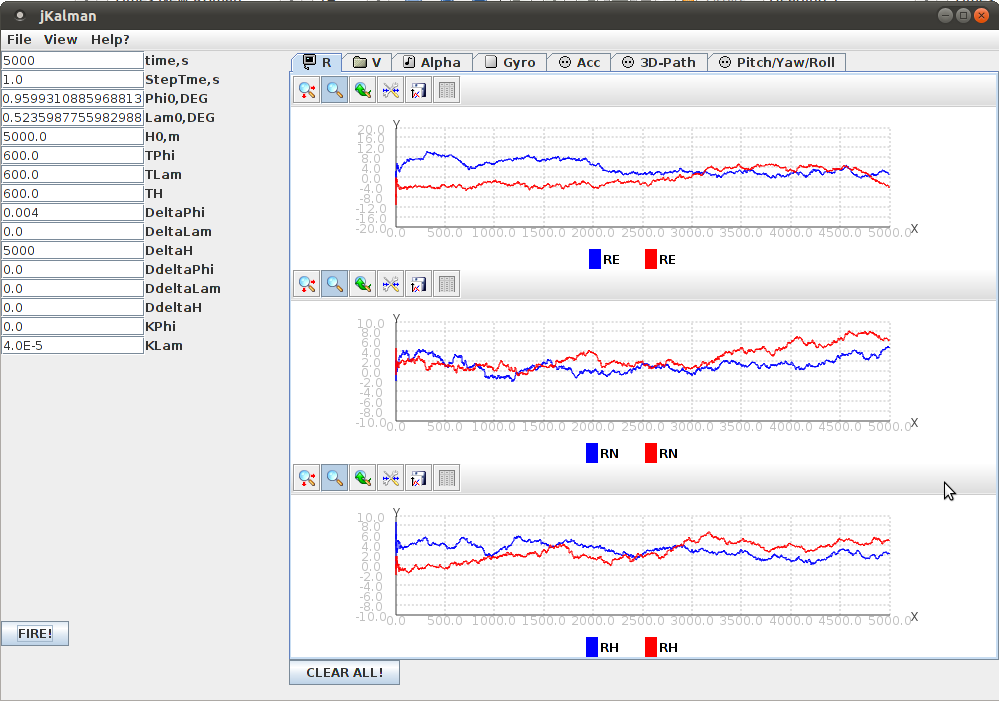
\includegraphics[scale=0.4]{r_soft}
\caption{Помилка оцінки координат}\label{fig:r_soft}
\end{figure}

\begin{figure}[t]
\centering
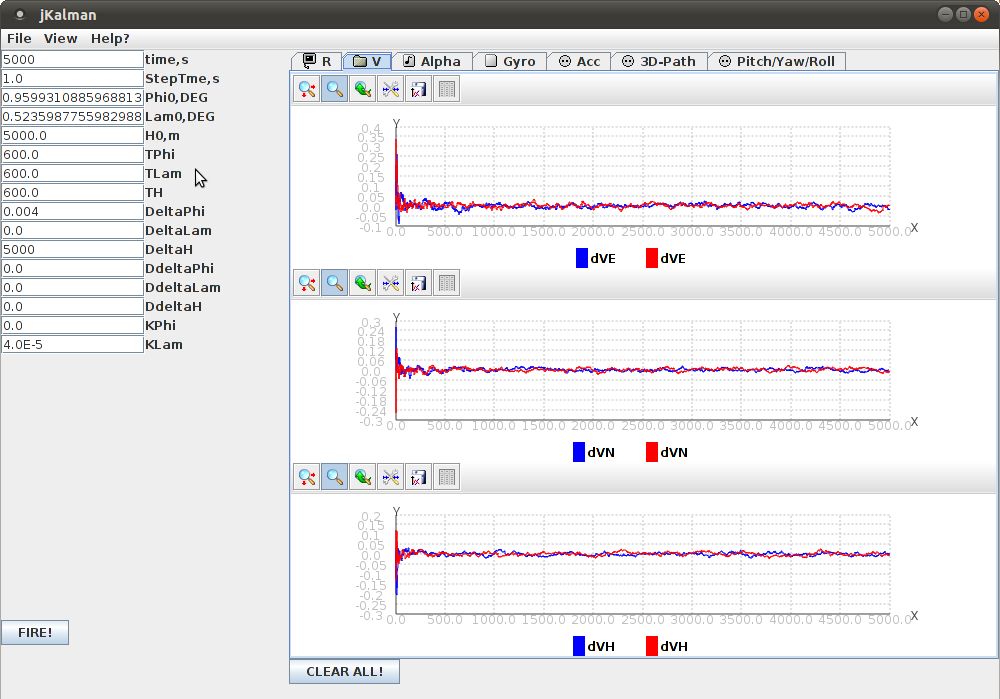
\includegraphics[scale=0.4]{v_soft}
\caption{Помилка оцінки швидкостей}\label{fig:v_soft}
\end{figure}

\begin{figure}[t]
\centering
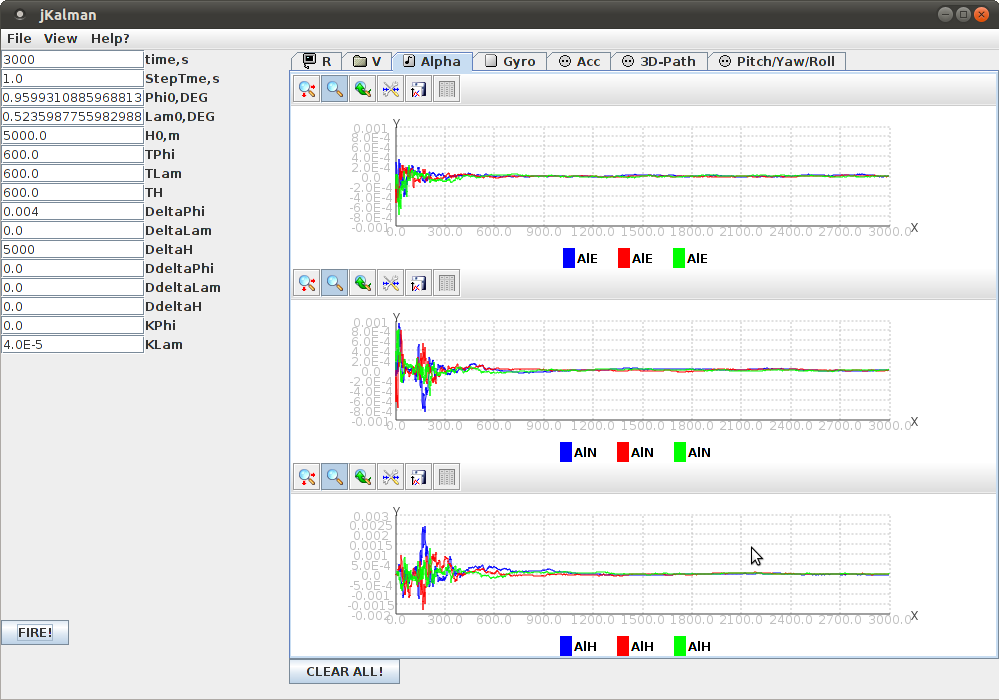
\includegraphics[scale=0.4]{alpha_soft}
\caption{Помилка оцінки координатного тригранника}\label{fig:alpha_soft}
\end{figure}


\begin{figure}[t]
\centering
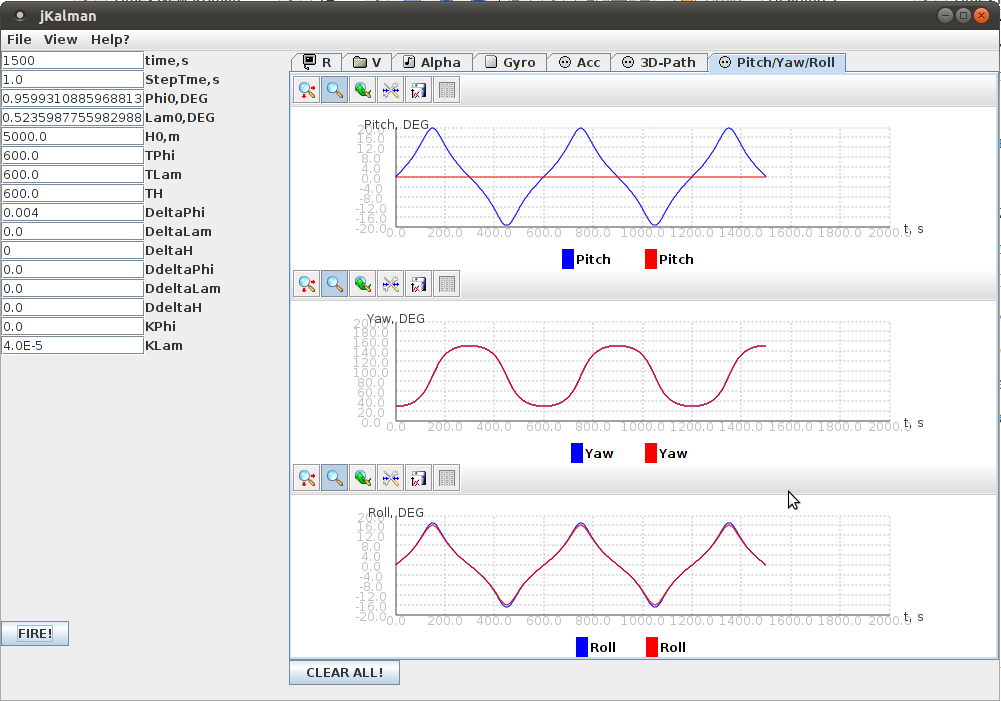
\includegraphics[scale=0.4]{pyr_soft}
\caption{Еволюція в часі кутового положення ЛА}\label{fig:pyr_soft}
\end{figure}


Графічна інформація зображається на спеціальних закладках з панеллю настроювання графіка. За допомогою панелі можна провести: зміщення, масштабування, поворот (для тривимірних зображень), настроїти колір та видимість лінії (Рис.\ref{fig:panel_3d_soft}).

\begin{figure}[t]
\centering
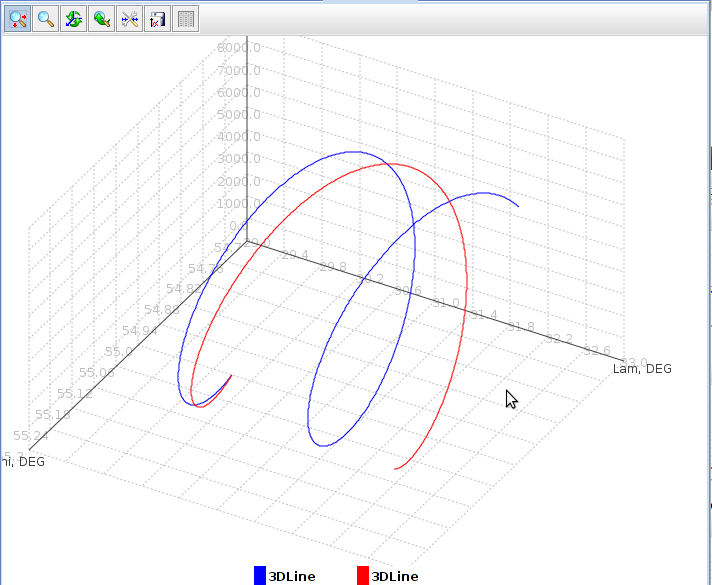
\includegraphics[scale=0.4]{panel_3d_soft}
\caption{Панель настроювання графіка}\label{fig:panel_3d_soft}
\end{figure}

На рис.\ref{fig:panel_data_soft} показане вікно редагування даних, за на основі яких будується графічне відображення. Звідси надається можливість скопіювати данні в буфер обміну, колір та видимість даних.

\begin{figure}[t]
\centering
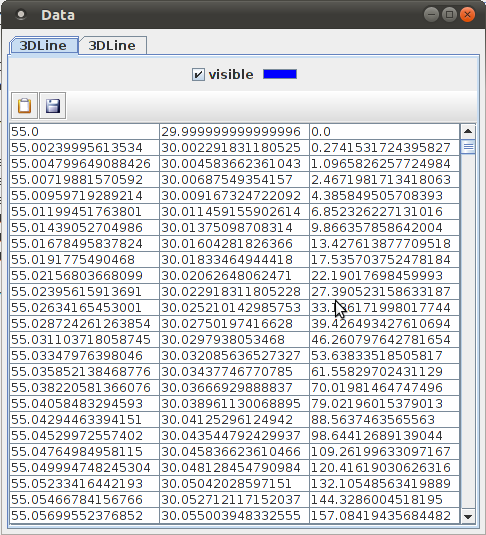
\includegraphics[scale=0.4]{panel_data_soft}
\caption{Панель настроювання графіка}\label{fig:panel_data_soft}
\end{figure}

\begin{figure}[t]
\centering
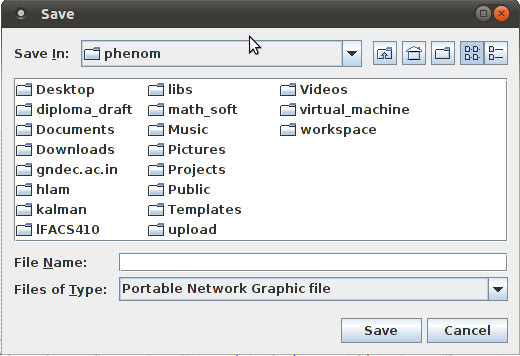
\includegraphics[scale=0.4]{panel_save_soft}
\caption{Панель настроювання графіка}\label{fig:panel_save_soft}
\end{figure}
Колір можливо змінити через спеціалізовані елементи керуванні за допомогою наступних діалогів: 
\begin{figure}[t]
\centering
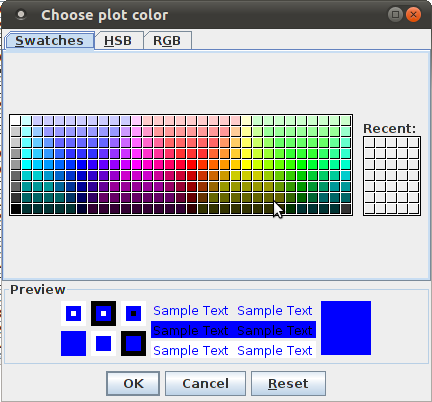
\includegraphics[scale=0.3]{panel_color1_soft}
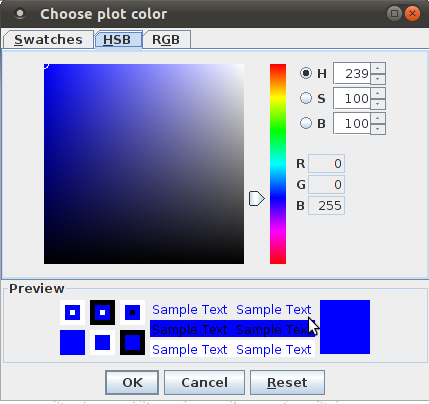
\includegraphics[scale=0.3]{panel_color2_soft}
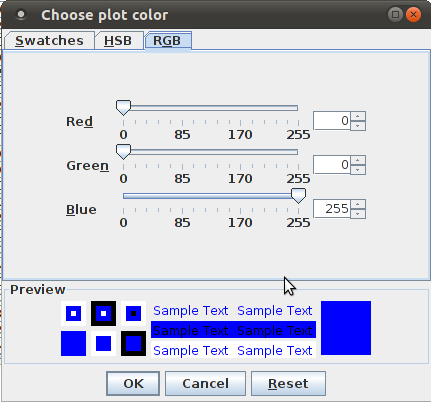
\includegraphics[scale=0.3]{panel_color3_soft}
\caption{Панель настроювання графіка}\label{fig:panel_color_soft}
\end{figure}

\subsection{Опис структури програми}

Програмне забезпечення створене на мові програмування Java, яка є обєктно орієнтовною мовою, основою якої є класи. В роботі роблені наступні класи:
\begin{itemize}
 \item FlightPathGen.class;
 \item RunISNS.class;
 \item jRKalman.class;
 \item InputsPanel.class;
 \item FlightPropPanel.class;
\end{itemize}

FlightPathGen.class -- генератор траєкторії руху ЛА та допоміжних функцій, крім конструктора включає наступні методи:

\begin{itemize}
 \item ComputePhiLamH() -- розраховує еволюцію координат;
 \item ComputeR1R2() -- розраховує параметри моделі Землі;
 \item ComputeV() -- розраховує швидкості руху ЛА;
 \item ComputeA() -- розраховує прискорення ЛА;
 \item ComputePRY() -- розраховує еволюцію кутового прискорення ЛА;
\end{itemize}


